Prompt engineering is the process of modifying the input of a model to achieve optimal results. In the case of large language models (LLMs), the prompt is a textual sequence indicating a task the model should perform, such as "In computer science, what is priority inversion?" - see Figure \ref{fig:priority-engineering}. Given this initial prompt, the information recovered from the LLMs will generally complete the task. However, it may not be in line with the intended audience. Engineering this prompt with modifiers can ensure that the response matches this target audience, such as "Respond in a way that a 5-year-old would understand: In computer science, explain what priority inversion is?" - see Figure \ref{fig:5-yo-prompt}.

An emerging property of LLMs enables prompt engineering: in-context learning (ICL). ICL is the ability of a language model to make inferences based on information provided with the input, typically preceding or following it. In the above example, given the proceeding prompt "Respond in a way that a 5-year-old would understand," the LLM would not update its parameters and respond using its pre-trained model but the context to shape the response.

\begin{figure}
    \centering
    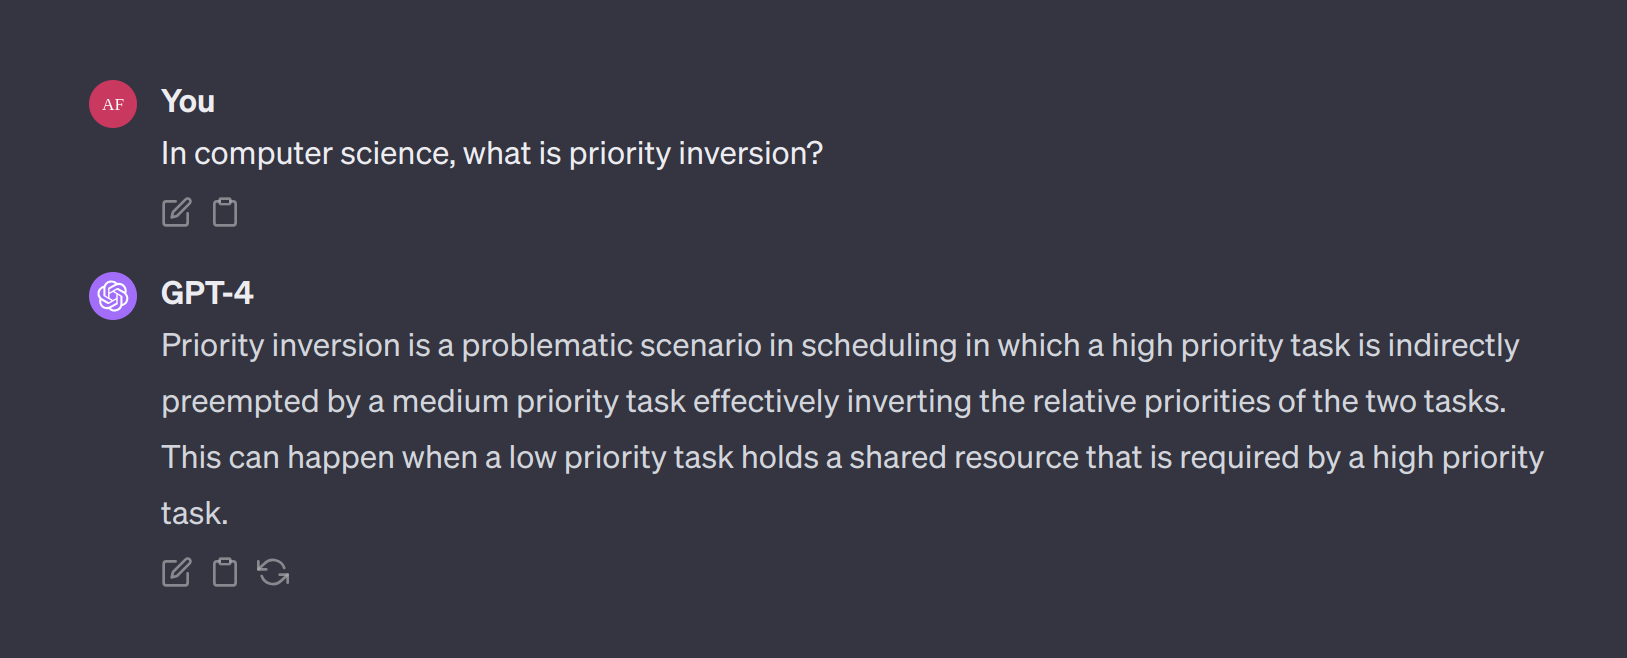
\includegraphics[width=1\linewidth]{sections//images/what-is-priority-inversion.png}
    \caption{Chat GPT asked a standard computer science question, using GPT 4.5}
    \label{fig:priority-engineering}
\end{figure}

\begin{figure}
    \centering
    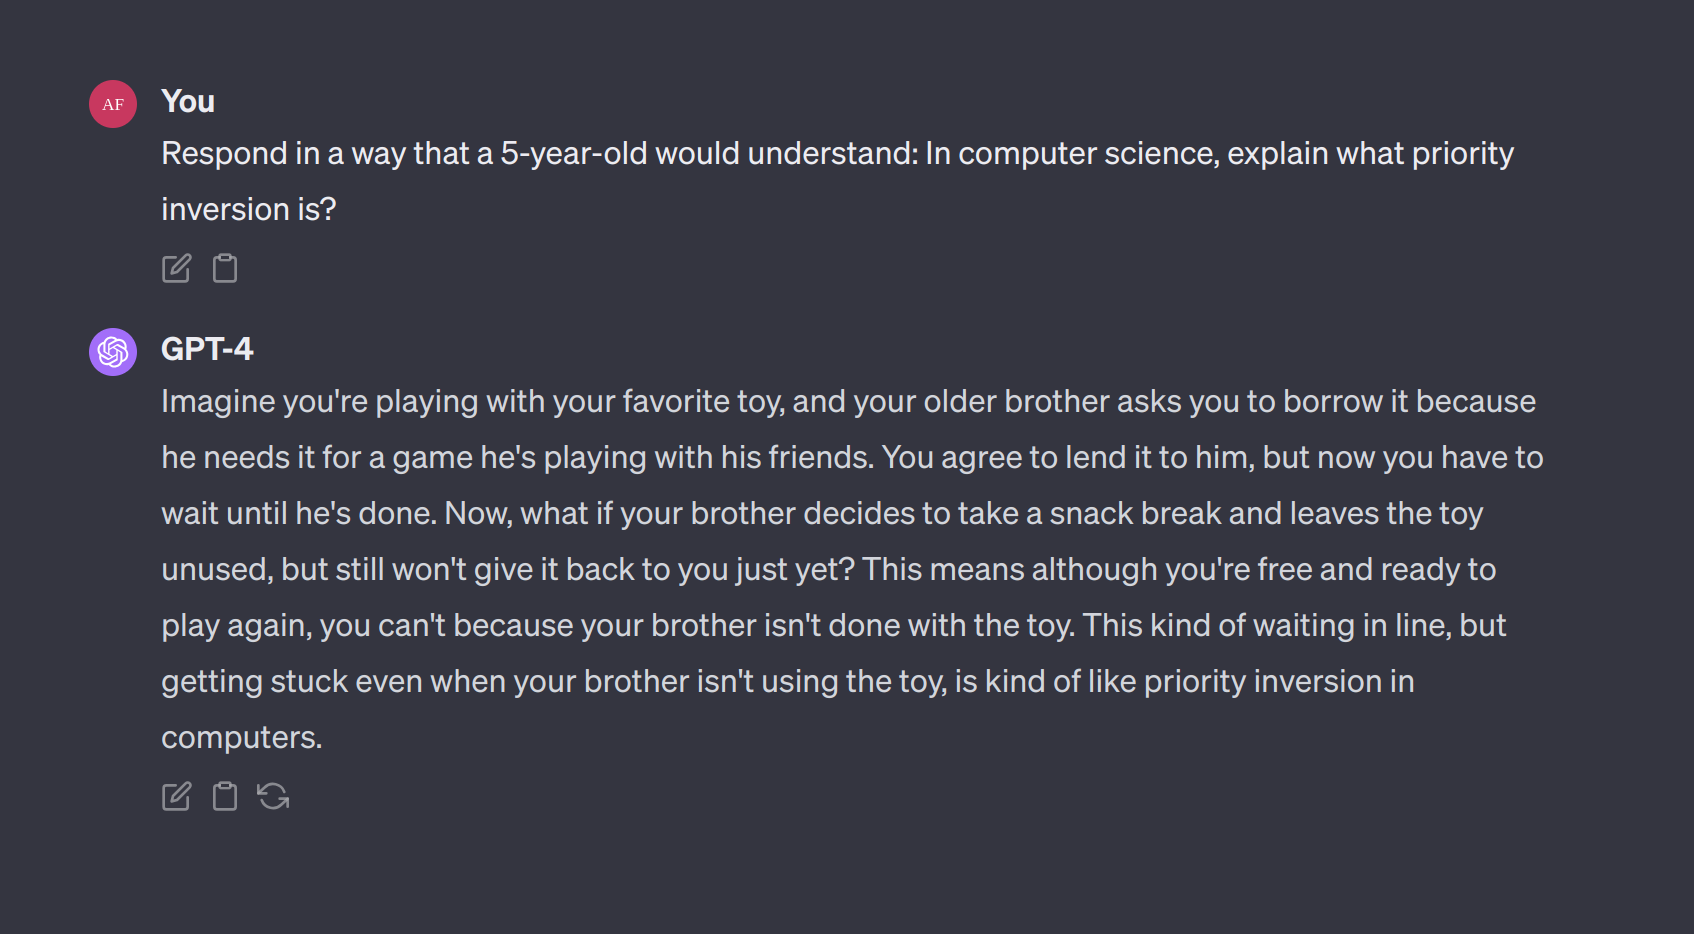
\includegraphics[width=1\linewidth]{sections//images/5-year-old-priority-inversion.png}
    \caption{Chat GPT asked a standard computer science question, with prompt engineering, using GPT 4.5}
    \label{fig:5-yo-prompt}
\end{figure}

Recently, Google released a new generative model, reportedly superior to the GPT-4 architecture, the Gemini model, in November 2023. Little research exists to evaluate the effect of prompt engineering on Gemini architecture.  

This research aims to understand whether prompt engineering improves the effects of downstream tasks presented within this mini-project and additionally establish some prompt-engineering performance comparison of GPT-4 to the Gemini model. 